\documentclass[runningheads]{llncs}

\usepackage[T1]{fontenc}
\usepackage{graphicx}
\usepackage{amsmath}
\usepackage{amssymb}
\usepackage{booktabs}
\usepackage{url}
\usepackage{placeins}

\setcounter{secnumdepth}{3}
\setlength{\textfloatsep}{8pt plus 2pt minus 2pt}
\setlength{\floatsep}{8pt plus 2pt minus 2pt}
\setlength{\intextsep}{8pt plus 2pt minus 2pt}

\begin{document}

\title{Robot Soccer Self-Localization with Active Inference}
\titlerunning{Robot Soccer Self-Localization}


\author{
Charel van Hoof\inst{1,2} \and
Noah van de Meer\inst{2} \and
Martijn Wisse\inst{1}
}

\authorrunning{C.A. van Hoof et al.}

\institute{
Department of Cognitive Robotics, Delft University of Technology, The Netherlands
\and
VDL Robotsports Team, The Netherlands
}

\maketitle
\begingroup
\renewcommand{\thefootnote}{\fnsymbol{footnote}}
\footnotetext[1]{The authors thank Geert Nijholt and other members of the VDL Robotsports MSL robot soccer team for their contributions.}
\endgroup

\begin{abstract}
This paper presents a continuous active-inference formulation of robot-soccer self-localization. The proposed method is efficient, robust, fast, and precise enough for RoboCup soccer. The continuous belief update combines prediction errors from motion and landmark observations. It leverages generalized coordinates in active inference, treating localization as a dynamically evolving belief whose higher-order motion terms, such as velocity and acceleration, directly shape prediction errors and belief updates, making the formulation well suited to fast-paced robot movement. Simulation experiments measure convergence over 1000 randomized trials per condition in static and moving-robot scenarios. In two-hour moving duration tests, the method maintained stable tracking under combined noise, dropout, a 110-degree field of view, and two-second landmark obstruction. Under landmark ambiguity with gated nearest-neighbor association, it also maintained stable tracking when initialized from a converged belief.
\keywords{Active inference \and Self-localization \and Robot soccer \and Predictive coding \and Generalized coordinates}
\end{abstract}

\section{Introduction}
\label{sec:introduction}

Robot soccer is a fast, real-world robotics domain where robust self-localization is an important prerequisite for useful play. A robot must therefore continuously estimate where it is on the field, with centimeter-level precision, from partial, intermittent, robot-perspective observations under a limited field of view while moving at high speed.

This work takes inspiration from biological navigation, where animals localize by combining self-motion cues with external spatial cues such as landmarks~\cite{tang_learning_2024},
suggesting a robot localization model in which motion input and landmark observations jointly maintain a latent belief about position on the field.
The generalized-coordinate formulation of active inference naturally integrates motion cues, such as velocity and acceleration, with landmark observations
in a shared belief over field pose. It thereby turns the biological intuition into a compact prediction-error minimization algorithm.

Active inference has been used as a framework for self-localization and navigation, but existing work does not provide a compact real-time localization formulation tailored to the fast-paced, centimeter-level requirements of robot soccer. For this setting, we derive a generalized-coordinate belief update on a known soccer field that combines motion and landmark prediction errors and reduces to compact matrix calculations that show a robust working solution in a simulation environment.

The paper makes the following contributions:
\begin{itemize}
    \item it formulates robot-soccer self-localization as generalized-coordinate active-inference belief updating on a known soccer field;
    \item it shows, in simulation experiments, that the resulting method is efficient, robust, fast, and precise enough for RoboCup soccer.
\end{itemize}

\section{Motivation and Requirement}
\label{sec:motivation-background}

The goal of our algorithm is to estimate the robot pose on the soccer field in the field coordinate system (FCS): position $x,y$ and orientation angle $\theta$. Observations are expressed in the robot coordinate system (RCS): odometry (velocity) and the IMU (acceleration) provide motion observations in $x,y$, and $\theta$, while visible landmarks, such as goals, corners, and the centre circle, are observed in $x$ and $y$, from which their bearing angle is calculated. With this information, the current belief represented in red in Fig.~\ref{fig:localization-requirement} must find the actual robot pose generating the observations in green.

\begin{figure}[!htbp]
    \centering
    \begin{minipage}[c]{0.45\linewidth}
        \centering
        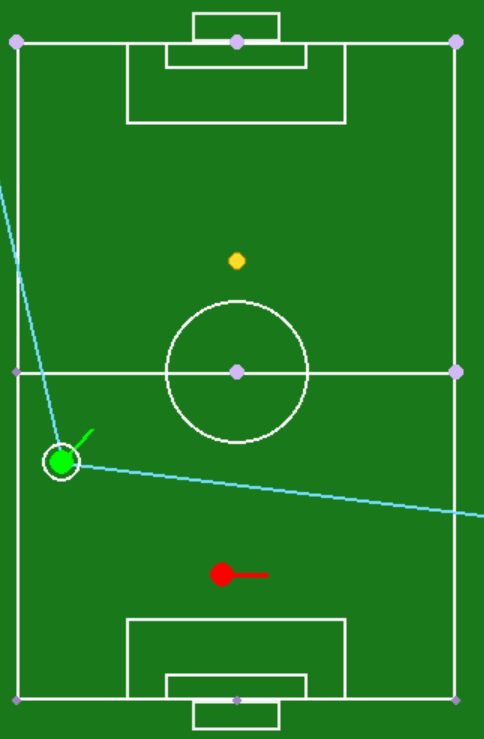
\includegraphics[width=0.58\linewidth]{figures/Soccer_field.png}
    \end{minipage}
    \hfill
    \begin{minipage}[c]{0.45\linewidth}
        \centering
        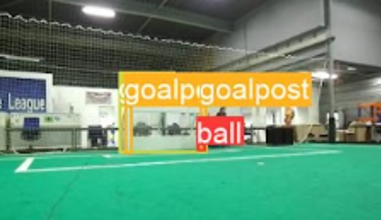
\includegraphics[width=0.62\linewidth]{figures/landmark1.png}\\[0.3em]
        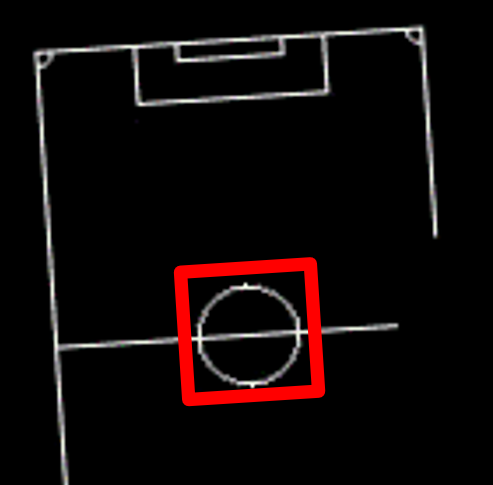
\includegraphics[width=0.25\linewidth]{figures/landmark2.png}
    \end{minipage}
    \caption{Robot-soccer localization requirement. The belief in red must converge to the actual pose generating the observations in green, using motion observations and visible landmarks as purple dots inside the limited field of view. Typical landmark examples include goal posts and the middle circle; the landmark center $(x,y)$ in RCS is used as input to the algorithm.}
    \label{fig:localization-requirement}
\end{figure}
This must be done for fast-moving robots, reaching speeds up to 5 m/s and accelerations up to 12 m/s$^2$. It must provide robust, centimeter-scale tracking despite noisy, partial, intermittent, and ambiguous landmark observations, including temporary obstruction and a restricted 110-degree field of view. The restricted field of view reflects RoboCup's evolution toward humanoid robot soccer, where omnivision cameras are not available, in line with RoboCup's long-term objective of developing fully autonomous humanoid robot soccer players capable of defeating the human World Cup champion by the middle of the 21st century~\cite{robocup_objective_2026}.
The method leverages the fact that robot soccer is played on a known field: landmarks are specified upfront and do not need to be learned, and the transformations between the robot coordinate system (RCS) and field coordinate system (FCS) are known.

\FloatBarrier

\section{Related Work}
\label{sec:related-work}

\subsection{Active Inference}
\label{subsec:related-active-inference-framing}

Active inference, the framework for minimizing the free energy, is rooted in the predictive-mind view that perception is an inference process: an agent maintains beliefs about hidden causes of sensory input and updates those beliefs by reducing prediction errors~\cite{hohwy_predictive_2013}. Under the free-energy principle, perception, learning, and action can be formulated as optimization of variational free energy, a tractable objective related to Bayesian model evidence~\cite{friston_free_2006,friston_free-energy_2009,friston_action_2010,friston_predictive_2009,parr_active_2022}. 
Within active inference, a common distinction is made between variational free energy (VFE), which is used for continuous-domain perception, state estimation, and reflex-like action, and expected free energy (EFE), which is used for discrete policy selection and planning~\cite{kaplan_planning_2018}. Our contribution builds on the VFE side of active inference, more specifically on perception and self-localization, not action.

In this paper, the hidden cause of interest is the robot's field pose, and the sensory evidence consists of motion and landmark observations. The VFE formulation represents this belief in generalized coordinates, including position, velocity, and acceleration. This makes it well suited to fast-paced movement estimation, because localization is treated as a dynamically evolving belief whose higher-order motion terms directly shape prediction errors and belief updates.

\subsection{Active-Inference Robotic Navigation}
\label{subsec:related-active-inference-navigation}

Active inference has already been used in robotic navigation contexts, with a focus on operating in environments for which no prior map is available. 
Catal et al.~\cite{catal_robot_2021} connect visual perception, path integration, localization, mapping, and navigation in a hierarchical active-inference model. However, they report that ``navigation is limited to the few trajectories that were tele-operated to build the map.'' Their evaluation shows topologically consistent mapping at 200 ms observation intervals, but does not report centimeter-level metric localization accuracy. 
De Tinguy et al.~\cite{de_tinguy_online_2025} take this further by learning the environment structure online while also planning through it. Their AIMAPP framework uses motion predictions and stored panoramic observations from a 360-degree sensory view, and reports drift-robust navigation with an $(x,y)$ RMSE of $1.83 \pm 0.77$ m in a controlled warehouse. This is useful for autonomous exploration, but it is not aimed at the RoboCup requirements defined in Section~\ref{sec:motivation-background}.

Free-energy-based state estimation has also been evaluated by Bos et al.~\cite{bos_free_2021} for a quadcopter under wind-induced colored noise, showing that generalized coordinates can be used effectively in robotic state estimation. 

These active-inference papers do not address the specific challenge identified in the previous section. Our contribution is therefore not a
general navigation system, but a fast and robust localization on a known soccer field.


\subsection{RoboCup and Humanoid Localization}
\label{subsec:related-robocup}

Classical localization methods for known robot-soccer fields commonly use Kalman-filter, particle-filter, or multi-hypothesis variants to combine motion prediction with visual landmark corrections.

Jochmann et al.~\cite{jochmann_efficient_2012} are the closest classical reference for the present setting because they address robust localization in humanoid RoboCup, where repeated field landmarks can create ambiguous observations and where relocalization is important. Their multi-hypothesis unscented Kalman-filter approach is therefore a strong existing solution for known-field robot-soccer showing the capability of localization under landmark ambiguity.

However, this existing solution does not address the specific formulation pursued in this paper. It remains a classical filter-based multi-hypothesis pose estimator, rather than a variational-free-energy formulation of self-localization. It estimates pose hypotheses without generalized-coordinate dynamics, whereas fast robot-soccer play motivates a belief state in which position, velocity, and acceleration are represented together. Its UKF-style estimator uses sigma-point propagation through the landmark model, which is more computationally intensive than an explicitly derived local geometric-Jacobian update. Its motion update is driven by motor commands or control input, whereas the formulation pursued here treats odometry and IMU measurements as motion prediction errors, grounding the update in observed rather than commanded movement. Finally, because Jochmann et al. show that multi-hypothesis localization is valuable for ambiguous landmarks, their work also motivates asking how far a compact single-belief formulation can remain stable before a multi-hypothesis extension becomes necessary.



\section{Method}
\label{sec:method}

\subsection{Variational Free Energy}
\label{subsec:first-principles}

The robot cannot directly observe its true field pose. It must infer a hidden state from sensory observations under a generative model. In Bayesian terms, the goal is to estimate a posterior belief over hidden state $x$ given observations $y$:
\begin{equation}
    p(x \mid y) =
    \frac{p(y \mid x)p(x)}{p(y)}.
    \label{eq:bayes}
\end{equation}
This posterior is generally intractable. Instead, a tractable belief $q(x;\zeta)$ is optimized so that it approximates the posterior over hidden state $x$. In active inference, this optimization is expressed as minimization of variational free energy, see Appendix~\ref{app:vfe-derivation}:
\begin{equation}
    \underset{\zeta}{\arg\min}\, \mathcal{F}(y,\zeta)
    =
    \underset{\zeta}{\arg\min}
    \int q(x;\zeta)
    \ln\left(
        \frac{q(x;\zeta)}{p(x,y)}
    \right) dx .
    \label{eq:vfe-general}
\end{equation}
The free-energy objective can be evaluated as a function of sensory data and belief-state parameters. It can therefore be minimized as an automatable optimization problem. Minimizing $\mathcal{F}(y,\zeta)$ with respect to $\zeta$ optimizes $q(x;\zeta)$ so that it approximates the posterior over hidden state $x$ given sensory observations $y$. For a Gaussian belief, as used in the Laplace approximation below, $\zeta$ corresponds to the mean and variance.
\subsection{Laplace-Encoded Free Energy}
\label{subsec:gaussian-errors}

Under the Laplace and mean-field approximations, the variational free energy in Eq.~\ref{eq:vfe-general} reduces to a sum of squared precision-weighted prediction errors; see Appendix~\ref{app:laplace-free-energy}. With belief parameters $\mu$, prediction error vector $\epsilon$, and precision matrix $\Pi$ (inverse variance), this gives
\begin{equation}
    \underset{\tilde{\mu}}{\arg\min}\, \mathcal{F}(y,\tilde{\mu})
    =
    \underset{\tilde{\mu}}{\arg\min}
    \left(
        \frac{1}{2}\tilde{\epsilon}^\top \tilde{\Pi} \tilde{\epsilon}
        -
        \frac{1}{2}\ln|\tilde{\Pi}|
    \right).
    \label{eq:vfe-gaussian}
\end{equation}
The tilde denotes generalized-coordinate quantities; in this paper, each pose variable is represented as a vector such as $\tilde{x}=[x,\dot{x},\ddot{x}]^\top$ for position, velocity, and acceleration. The compact formulation in Eq.~\ref{eq:vfe-gaussian} can be unpacked for our non-hierarchical robot-soccer model as:

\begin{align}
    \underset{\mu}{\arg\min}\, \mathcal{F}(y,\mu)
    &=
    \underset{\mu}{\arg\min}
    \Bigg[
    \frac{1}{2}
    \sum_{j=1}^{P+1}
    \sum_{k=1}^{n}
    \left(
        \Pi_{g(i,j,k)}
        \epsilon^2_{g(i,j,k)}
        -
        \ln\left(\Pi_{g(i,j,k)}\right)
    \right)
    \nonumber \\
    &\qquad\qquad+
    \frac{1}{2}
    \sum_{j=1}^{P+1}
    \sum_{k=1}^{q}
    \left(
        \Pi_{p(i,j,k)}
        \epsilon^2_{p(i,j,k)}
        -
        \ln\left(\Pi_{p(i,j,k)}\right)
    \right)
    \Bigg].
    \label{eq:vfe-motion-place-expanded}
\end{align}

The first term contains the motion prediction errors $g$. The hidden state is one robot field-pose belief with three pose variables, $x$, $y$, and $\theta$, so $n=3$. Each pose variable is represented up to second order in generalized coordinates, namely position, velocity, and acceleration, so $P=2$. This gives 9 motion prediction errors to be minimized.

The second term contains the sensory landmark prediction errors $p$. In this paper the landmarks are static (only position, no speed or acceleration), and up to 9 landmarks are used, giving 27 precision-weighted landmark prediction errors to be minimized.


\medskip
Free energy is therefore low when one field-pose belief is jointly consistent with the robot's motion evidence and its observed field landmarks. Minimizing the free energy means finding the three generalized-coordinate belief vectors $\tilde{\mu}_{g,x}$, $\tilde{\mu}_{g,y}$, and $\tilde{\mu}_{g,\theta}$, or nine scalar belief parameters in total, that minimize these 36 prediction errors. This minimization is done by gradient descent.

\subsection{Gradient Descent on the Free Energy}
\label{subsec:gradient-descent-free-energy}

 Taking the free-energy gradient with respect to $\tilde{\mu}_{g}$ gives the generalized-coordinate belief update, see Appendix~\ref{app:slide15-update-derivation}:
\begin{equation}
    \dot{\tilde{\mu}}_{g}
    =
    D\tilde{\mu}_{g}
    +
    \underbrace{
        \left[
            -
            D^\top \tilde{\Pi}_{g}\tilde{\epsilon}_{g}
            +
            \left(
                \partial_{\tilde\mu_g}\tilde{f}(\tilde{\mu}_{g})
            \right)^\top
            \tilde{\Pi}_{g}\tilde{\epsilon}_{g}
        \right]
    }_{\text{motion prediction errors}}
    +
    \underbrace{
        \sum_{\mathrm{landmarks}}
        \left(
            \partial_{\tilde\mu_g}\tilde{g}(\tilde{\mu}_{g})
        \right)^\top
        \tilde{\Pi}_{p}\tilde{\epsilon}_{p}
    }_{\text{landmark prediction errors}}.
    \label{eq:slide15-generic-update}
\end{equation}
with prediction errors
\begin{equation}
    \tilde{\epsilon}_g
    =
    D\tilde{\mu}_g
    -
    \tilde{f}(\tilde{\mu}_g),
    \qquad
    \tilde{\epsilon}_p
    =
    \tilde{y}
    -
    \tilde{g}(\tilde{\mu}_g).
    \label{eq:prediction-errors}
\end{equation}

\subsubsection{Motion Part}
\label{subsec:gradient-motion}

The motion part of Eq.~\ref{eq:slide15-generic-update} is the motion prediction-error contribution.
To keep the notation compact, the following equations show the $x$ component, $\tilde{\mu}_{g,x}=[\mu_{g,x},\mu'_{g,x},\mu''_{g,x}]^\top$, which is the robot's generalized-coordinate belief for its field $x$ position in the Field Coordinate System (FCS). Likewise for $y$ and $\theta$.
\begin{align}
    \tilde{\epsilon}_{g,x}
    &=
    D\tilde{\mu}_{g,x}
    -
    \tilde{f}(\tilde{\mu}_g)_x
    =
    \begin{bmatrix}
        \mu'_{g,x} \\
        \mu''_{g,x} \\
        0
    \end{bmatrix}
    -
    \begin{bmatrix}
        f_{\mathrm{RCS}\rightarrow\mathrm{FCS}}(v^{\mathrm{odom}})_x \\
        f_{\mathrm{RCS}\rightarrow\mathrm{FCS}}(a^{\mathrm{IMU}})_x \\
        0
    \end{bmatrix}
    \nonumber \\
    &=
    \text{motion belief in FCS}
    -
    \text{predicted motion in FCS}.
    \label{eq:motion-error-x}
\end{align}
Here, $D$ is the generalized-coordinate shift operator: it shifts the vector entries up by one and adds a zero at the bottom.
The term $\tilde{f}$ is the motion generative model. In this implementation, we choose to use the available sensory odometry and IMU measurements directly, rather than motor commands or a separate movement function. To make use of these motion sensory observations, they are translated from RCS into FCS. Since the soccer-field geometry is known, this is a straightforward RCS-to-FCS translation using the belief heading, see Appendix~\ref{app:coordinate-conventions}, and the same transform is used for both velocity and acceleration observations.
The corresponding motion precision matrix for the $x$ component is
\begin{equation}
    \tilde{\Pi}_{g,x}
    =
    \begin{bmatrix}
        \Pi_{\mathrm{odo}} & 0 & 0 \\
        0 & \Pi_{\mathrm{IMU}} & 0 \\
        0 & 0 & 0
    \end{bmatrix},
    \label{eq:motion-precision-x}
\end{equation}
which contains the precisions of the odometry and IMU prediction errors. In this implementation these precisions are fixed parameters and set to 1, and they can be tuned if required. Motion in $x$, $y$, and $\theta$ is treated as factorized, matching the robot-soccer setting where omnidirectional wheels or humanoid stepping can produce independent motion components. As a design choice, the term $\left(\partial_{\tilde\mu_g}\tilde{f}(\tilde{\mu}_g)\right)^\top$ is zero because the motion is not dependent on the current field position or angle.

\subsubsection{Landmark Part}
\label{subsec:gradient-landmarks}

The landmark part of Eq.~\ref{eq:slide15-generic-update} is the sensory prediction-error contribution.
To keep the notation compact, the following equations show the x coordinate of one unambiguous observed landmark example.
\begin{align}
    \tilde{\epsilon}_{p,x}
    &=
    \begin{bmatrix}
        y_x \\
        0 \\
        0
    \end{bmatrix}
    -
    \begin{bmatrix}
        g_{\mathrm{FCS}\rightarrow\mathrm{RCS}}(\mu_g)_x \\
        0 \\
        0
    \end{bmatrix}
    \nonumber \\
    &=
    \text{observed landmark in RCS}
    -
    \text{predicted landmark in RCS}.
    \label{eq:landmark-error-x}
\end{align}
Here, $y_x$ is the observed landmark $x$ position in RCS and $g_{\mathrm{FCS}\rightarrow\mathrm{RCS}}(\mu_g)_x$ is the predicted landmark $x$ position in RCS. The same construction is used for the observed landmark $y$ position and $\theta$ angle.
Landmark observations provide relative $x$ and $y$ positions, not relative velocity or acceleration, so there are no generalized-coordinate rows for landmark velocity or acceleration in the sensory prediction error.
The soccer field geometry is predefined, so the landmark observation model and its Jacobian can be calculated straightforwardly from the known FCS/RCS coordinate conventions, see Appendix~\ref{app:coordinate-conventions}.
The term $\partial_{\tilde\mu_g}\tilde{g}(\tilde{\mu}_g)$ in Eq.~\ref{eq:slide15-generic-update} is the landmark Jacobian $\boldsymbol{J}_{\ell}$. It describes how small changes in the robot pose, including $x$, $y$, and $\theta$, affect the predicted landmark observation.

For the observed landmark $x$ coordinate, the corresponding landmark precision matrix is
\begin{equation}
    \tilde{\Pi}_{p,x}
    =
    \begin{bmatrix}
        \Pi_{\mathrm{cam}} & 0 & 0 \\
        0 & 0 & 0 \\
        0 & 0 & 0
    \end{bmatrix}.
    \label{eq:landmark-precision-x}
\end{equation}

\subsection{Distance-Weighted Precision Modifier}
\label{subsec:distance-weighted-precision}

A useful optional refinement is to make landmark precision depend on observation distance. Camera-based position estimates generally become less precise at longer distances because the pixel-per-meter ratio decreases with range. Distance weighting provides a simple way to represent this range-dependent confidence in the landmark update. It is not required for convergence: suitable learning-rate settings can also yield stable behavior. As a practical design choice, we use a precision distance modifier based on the landmark's predicted position in RCS:

\begin{equation}
d_\ell =
\sqrt{
    \left(g(\mu_g)_{x,\ell}\right)^2
    +
    \left(g(\mu_g)_{y,\ell}\right)^2
},
    \qquad
    \rho_\ell
    =
    \max
    \left(
        \rho_{\min},
        \frac{1}{1 + \left(d_\ell / d_{\mathrm{ref}}\right)^2}
    \right).
    \label{eq:distance-precision-modifier}
\end{equation}
In the proof-of-concept experiments, $d_{\mathrm{ref}}=600$ cm and $\rho_{\min}=0.15$.

\subsection{Resulting Update Rules}
\label{subsec:update-rules}

For the $x$ field-pose component, this gives the following straightforward
matrix calculation. Here, $\boldsymbol{J}_{g_x,\ell}$ is the column of the landmark Jacobian associated with belief component $g_x$, and the scalar factors $\eta^{c}_{xy}$, $\eta^{v}_{xy}$, and $\eta^{a}_{xy}$ denote learning rates for the camera, odometry-velocity, and IMU-acceleration update terms.

{
\small
\begin{align}
\dot{\tilde{\boldsymbol{\mu}}}_{g_x}
&\!=\!
\begin{bmatrix}
\mu'_{g_x}\\
\mu''_{g_x}\\
0
\end{bmatrix}
\!-\!
\begin{bmatrix}
0\\
\eta^{v}_{xy}\Pi_{\mathrm{odo}}
\left(\mu'_{g_x}-f(v^{\mathrm{odom}})_x\right)\\
\eta^{a}_{xy}\Pi_{\mathrm{IMU}}
\left(\mu''_{g_x}-f(a^{\mathrm{IMU}})_x\right)
\end{bmatrix}
\!+\!
\sum_{\ell}
\begin{bmatrix}
\eta^{c}_{xy}
\rho_\ell \boldsymbol{J}_{g_x,\ell}^{\top}
\boldsymbol{\Pi}_{\mathrm{cam}}
\left(y_{x,\ell}-g(\mu_g)_{x,\ell}\right)\\
0\\
0
\end{bmatrix}.
\end{align}
}
The same calculation is applied to the $y$ and $\theta$ belief components using their corresponding landmark-Jacobian columns and learning rates. The resulting generalized-coordinate update is integrated with Euler's forward method using a configurable step size corresponding to the frequency of the robot localization loop. The learning rates are manually tuned. The update has a simple intuition. First, the motions of the current generalized coordinates are shifted forward in time. Then the motion terms correct the belief: if the predicted movement is too fast, the acceleration is reduced. Next, the landmark terms correct the belief: If the position is too far, the velocity is reduced.

 The resulting update rules are efficient matrix calculations over $x$, $y$, and $\theta$, suitable for a high-frequency robot-soccer localization loop.

\section{Simulation Experiments and Results}
\label{sec:experiments}
The simulation code is supplied with the paper \cite{code_active_inference_2026} so that readers can reproduce the experiments, vary the conditions, and inspect the resulting localization behavior directly.

This section is organized as a progression toward a real-robot test environment. This is evaluated in two complementary ways. First, convergence scenarios use many randomized trials to test whether the belief can recover from different initial field positions and reach centimeter-level localization without landmark ambiguity. Next, tracking scenarios test whether the belief remains stable over time while the robot moves under noise, dropout, limited field of view, obstruction, and landmark ambiguity.
\footnote{Simulations were run on a modest 11th Gen Intel Core i5-1135G7 laptop (2.40 GHz, 4 cores). The simulation required approximately 82 µs/step, corresponding to 12,200 steps/s. This is an indicative hardware-dependent measurement, not a benchmark.}
\begin{figure}[t]
    \centering
    \begin{minipage}[t]{0.55\linewidth}
        \vspace{0pt}
        \centering
        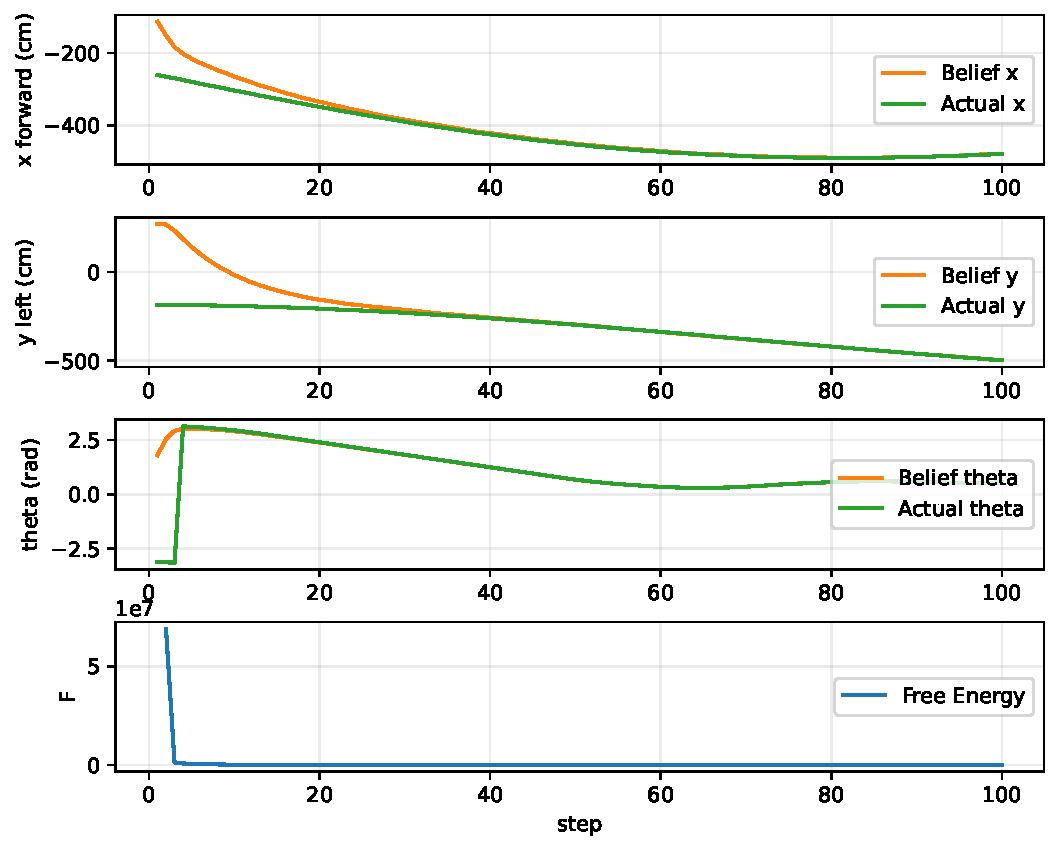
\includegraphics[width=0.95\linewidth,page=1]{figures/paper_experiment_20260909_172050.pdf}\\
        \small (a) Position tracking
    \end{minipage}
    \hfill
    \begin{minipage}[t]{0.42\linewidth}
        \vspace{0pt}
        \centering
        \includegraphics[width=0.95\linewidth,page=2]{figures/paper_experiment_20260909_172050.pdf}\\
        \small (b) Velocity traking

        \vspace{0.25em}

        \includegraphics[width=0.95\linewidth,page=3]{figures/paper_experiment_20260909_172050.pdf}\\
        \small (c) Acceleration tracking
    \end{minipage}
    \caption{\scriptsize Representative moving-robot belief estimate with noisy observations. Starting from random belief and actual poses, the belief converges to and tracks the actual pose in FCS as the robot follows a circular path. In (a), position and orientation are not observed directly; visible landmarks are observed in RCS $x$ and $y$, with bearing derived from these observations. In (b) and (c), velocity and acceleration observations in RCS are transformed to FCS using the belief heading. These plots illustrate that the update estimates generalized-coordinate dynamics rather than only pose.}
    \label{fig:typical-experiment-results}
\end{figure}
\FloatBarrier

\subsection{Static Robot Scenarios}
\label{subsec:experiments-static}

We first verify basic static convergence and progressively increase scenario complexity in subsequent sections. Here, the pose is inferred from unambiguous landmarks alone.
Table~\ref{tab:static-convergence-results} shows 100\% convergence from nearby and random initial positions, with varying numbers of visible landmarks and with or without dropout, noise, or both. In the near-start condition with 9 visible landmarks, convergence required only $23.6 \pm 5.0$ inference steps. Fewer available landmarks, noise or obstruction increased the number of inference steps needed for convergence.

\begin{table}[!htbp]
    \centering
    \caption{\scriptsize 100\% static robot convergence across a representative set covering nearby and random initial positions, varying visible landmark counts, and optional noise and dropout, using unique-ID data association. A trial is successful when the belief reaches the actual pose within 3 cm positional error and 3 degrees orientation error for at least five consecutive inference steps. Random: actual and initial belief poses sampled independently across the field, testing captured-robot-style recovery from an arbitrary wrong pose. Near: initial belief offset from the actual pose by at most 50 cm in x/y and 20 degrees in heading. Landmark-position noise in centimeters, landmark-angle noise in degrees.}
    \label{tab:static-convergence-results}
    \scriptsize
    \begin{tabular}{rrrrrlllll}
        \toprule
        N & Success & Mean & SD & P99 & Start & LM & Hz & Noise & Drop \\
        \midrule
        1000 & 100\% & 55.8 & 19.1 & 132 & Random & 9 & 40 & None & None \\
        1000 & 100\% & 23.6 & 5.0 & 36 & Near & 9 & 40 & None & None \\
        1000 & 100\% & 45.9 & 14.4 & 101 & Random & 9 & 200 & None & None \\
        1000 & 100\% & 63.9 & 22.1 & 149 & Random & 9 & 40 & 10 & 10\% \\
        1000 & 100\% & 129.4 & 85.3 & 467 & Random & 5 & 40 & None & None \\
        1000 & 100\% & 259.8 & 105.4 & 609 & Random & 2 & 40 & None & None \\
        1000 & 100\% & 48.2 & 20.4 & 113 & Near & 5 & 40 & 10 & 10\% \\
        1000 & 100\% & 112.0 & 40.7 & 225 & Near & 2 & 40 & 10 & 10\% \\
        \bottomrule
    \end{tabular}
\end{table}

\FloatBarrier

\subsection{Dynamic Robot Scenarios}
\label{subsec:experiments-dynamic}

The next question is whether the algorithm can converge while the actual robot is moving. Table~\ref{tab:dynamic-convergence-results} shows 100\% convergence across all tested dynamic scenarios. In the near-start condition with 9 visible landmarks, convergence required $44.2 \pm 22.4$ inference steps. The moving-robot results follow the same main trend as the static tests: fewer available landmarks, noise and obstruction increase the number of inference steps needed for convergence, but do not prevent recovery in these tests with unambiguous landmarks.
\footnote{For a kidnapped-robot-style recovery with only two unique landmarks visible at 40 Hz, 260 steps correspond to 6.5 s in the static case and 388 steps to 9.7 s in the dynamic case, which remains practical for recovery.}
The representative noisy run in Fig.~\ref{fig:typical-experiment-results} illustrates this behavior. The belief starts away from the actual pose, is corrected by motion and landmark prediction errors, and then remains close to the moving actual robot. The velocity and acceleration plots show that the update estimates a generalized-coordinate belief rather than only a static pose.

\begin{table}[!htbp]
    \centering
    \caption{\scriptsize 100\% dynamic-robot convergence. The robot follows random target trajectories, reaching speeds up to 5 m/s and accelerations up to 12 m/s$^2$. Tests use the same near/random starting position, landmark-visibility, noise, unique-ID data association, and dropout conditions as Table~\ref{tab:static-convergence-results}.}
    \label{tab:dynamic-convergence-results}
    \scriptsize
    \begin{tabular}{rrrrrlllll}
        \toprule
        N & Success & Mean & SD & P99 & Start & LM & Hz & Noise & Drop \\
        \midrule
        1000 & 100\% & 61.4 & 19.0 & 119 & Random & 9 & 40 & None & None \\
        1000 & 100\% & 44.2 & 22.4 & 105 & Near & 9 & 40 & None & None \\
        1000 & 100\% & 53.5 & 22.8 & 140 & Random & 9 & 200 & None & None \\
        1000 & 100\% & 74.9 & 28.2 & 163 & Random & 9 & 40 & 10 & 10\% \\
        1000 & 100\% & 121.2 & 57.4 & 308 & Random & 5 & 40 & None & None \\
        1000 & 100\% & 388.5 & 248.8 & 1313 & Random & 2 & 40 & None & None \\
        1000 & 100\% & 93.6 & 60.5 & 267 & Near & 5 & 40 & 10 & 10\% \\
        1000 & 100\% & 289.4 & 234.6 & 1157 & Near & 2 & 40 & 10 & 10\% \\
        \bottomrule
    \end{tabular}
\end{table}
\FloatBarrier

\subsection{Tracking Duration Test}
\label{subsec:experiments-visibility-stress}

Tracking duration tests shift the focus from convergence to sustained tracking under partial and interrupted landmark visibility. To approximate humanoid robot-soccer perception, landmark visibility is restricted to a representative 110-degree field of view, and the simulation includes 2-second obstruction periods in which other robots temporarily block relevant field landmarks.

Under the combined conditions of noise, dropout, limited field of view, and temporary obstruction, the method remained stable over a 2-hour Random targets run initialized from a near-start belief. The result is not error-free tracking at every instant, but stable recovery: motion terms keep the belief evolving during weak landmark evidence, and later landmark observations correct accumulated deviations. Table~\ref{tab:visibility-stress-tracking-summary} summarizes this behavior. The left panel reports the percentage of timesteps within each error threshold; the right panel shows that more visible landmarks correlate with lower mean absolute X error. Appendix~\ref{sec:appendix-landmark-tracking} provides a more detailed view of how landmark availability affects tracking error over time.

\begin{table}[!htbp]
    \centering
    \caption{\scriptsize Sustained tracking under challenging visibility conditions, demonstrated over two continuous hours at speeds up to5~m/s and accelerations up to 12~m/s$^2$, with observation noise, landmark dropout, a $110^\circ$ field of view, and temporary obstruction. The near-start Random targets run uses unique-ID landmark association at 40 Hz with 9 landmarks; while moving, the robot heading continuously rotates toward (300 cm, 0 cm). The run contains 288,000 inference timesteps (2 h at 40 Hz). Left: percentage of timesteps within each error threshold. For example, 39.44\% in the \(|x|\) column means that the absolute \(x\)-position error was at most 3 cm for 39.44\% of the timesteps. Right: Mean absolute X error, SD, and percentage of timesteps by visible landmark count during the two-hour tracking run. More visible landmarks correlate with lower error.}
    \label{tab:visibility-stress-tracking-summary}
    \scriptsize
    \begin{minipage}[t]{0.49\linewidth}
        \centering
        \textbf{(a) Tracking precision}\\[0.25em]
        \setlength{\tabcolsep}{5pt}
        \begin{tabular}{lccc}
            \toprule
            Band & $|x|$ & $|y|$ & $|\theta|$ \\
            \midrule
            3 cm / 1 deg & 39.44\% & 31.50\% & 94.25\% \\
            5 cm / 2 deg & 61.07\% & 50.26\% & 98.83\% \\
            7.5 cm / 3 deg & 79.64\% & 68.86\% & 99.69\% \\
            10 cm / 4 deg & 90.12\% & 81.73\% & 99.93\% \\
            15 cm / 5 deg & 97.86\% & 94.88\% & 99.99\% \\
            20 cm / 7.5 deg & 99.59\% & 98.73\% & 100.00\% \\
            25 cm / 10 deg & 99.90\% & 99.73\% & 100.00\% \\
            30 cm / 15 deg & 99.98\% & 99.96\% & 100.00\% \\
            \bottomrule
        \end{tabular}
    \end{minipage}
    \hfill
       \begin{minipage}[t]{0.49\linewidth}
        \centering
       \textbf{(b) X error by visible landmarks}\\[0.25em]
\setlength{\tabcolsep}{3pt}
\begin{tabular}{lccc}
    \toprule
    Visible LM & Mean $|x|$ (cm) & SD & Timestep \% \\
    \midrule
    0 & 6.38 & 5.13 & 0.12 \\
    1 & 5.83 & 4.76 & 1.77 \\
    2 & 5.55 & 4.55 & 8.11 \\
    3 & 5.28 & 4.20 & 16.88 \\
    4 & 4.92 & 3.93 & 27.32 \\
    5 & 4.58 & 3.66 & 25.56 \\
    6 & 4.13 & 3.19 & 15.09 \\
    7 & 4.00 & 3.20 & 3.34 \\
    8 & 3.83 & 2.94 & 1.44 \\
    9 & 3.46 & 2.67 & 0.35 \\
    \bottomrule
\end{tabular}
    \end{minipage}
\end{table}

\FloatBarrier

\subsection{Tracking Duration Test Under Landmark Ambiguity}
\label{subsec:experiments-landmark-ambiguity}

The next stress condition tests landmark ambiguity. Many soccer-field landmarks are geometrically repeated, so a local observation does not always identify a unique field location. For example, an observed field corner can correspond to any of the four physical field corners. This creates a data-association problem: the algorithm must decide which known FCS landmark generated the RCS observation before the prediction error can be used for belief updating.

In this proof of concept, ambiguity is handled with gated nearest-neighbor association. For each observed landmark type, candidate map landmarks of the same type are projected into RCS from the current belief; the closest candidate is selected only if its prediction error falls within a gating threshold. Otherwise, the observation is rejected for that update step. This is a deliberately simple and pragmatic association strategy. Although more advanced multi-hypothesis approaches were considered, the simulations showed that gated nearest-neighbor matching was sufficient for the present proof of concept. With landmark ambiguity enabled, the method maintained stable tracking when initialized from a converged belief.


\begin{table}[!htbp]
    \centering
    \caption{\scriptsize Sustained tracking under the challenging conditions of
Table~\ref{tab:visibility-stress-tracking-summary}, with landmark ambiguity.}
    \label{tab:landmark-ambiguity-tracking}
    \scriptsize
    \setlength{\tabcolsep}{5pt}
    \begin{tabular}{lccc}
        \toprule
        Band & $|x|$ & $|y|$ & $|\theta|$ \\
        \midrule
        3 cm / 1 deg & 39.05\% & 31.37\% & 94.00\% \\
        5 cm / 2 deg & 60.09\% & 50.21\% & 98.82\% \\
        7.5 cm / 3 deg & 78.71\% & 68.57\% & 99.71\% \\
        10 cm / 4 deg & 89.69\% & 81.74\% & 99.93\% \\
        15 cm / 5 deg & 97.67\% & 94.63\% & 99.98\% \\
        20 cm / 7.5 deg & 99.58\% & 98.47\% & 100.00\% \\
        25 cm / 10 deg & 99.97\% & 99.65\% & 100.00\% \\
        30 cm / 15 deg & 100.00\% & 99.93\% & 100.00\% \\
        \bottomrule
    \end{tabular}
\end{table}
\FloatBarrier

\section{Discussion}
\label{sec:discussion}
Although the simulations demonstrate robust tracking in the tested conditions, several limitations and natural extensions remain for real-robot evaluation:
\begin{itemize}
    \item Jochmann et al.~\cite{jochmann_efficient_2012} motivate multi-hypothesis localization for ambiguous RoboCup settings. The present simulations show that tracking with a single belief state is possible, but real-robot testing in match conditions should determine whether a multi-hypothesis active-inference extension is necessary.
    \item The approach relies on reliable landmark detection, which shifts part of the problem to the perception pipeline. However, mature object-detection methods such as YOLO can reliably provide suitable landmark candidates for the inference algorithm.
    \item The soccer field is symmetric, so the robot may need an additional source of unique information to resolve mirror-image pose hypotheses reliably. Possible symmetry-breaking cues include a noisy compass cue, an external landmark outside the field, or an initialization routine.
    \item Future work will include benchmarking the proposed approach against Kalman-filter-based localization on a physical robot.
    \item The algorithm could be extended with adaptive precision learning, active inference provides mechanisms to learn the precision of prediction errors, for example to detect degrading sensors.
    \item The algorithm could be extended to handle different frequencies for different sensory streams, for example accommodating higher-frequency IMU observations and lower-frequency camera-based landmark detections.
\end{itemize}

\section{Conclusion}
\label{sec:conclusion}

This paper presented an active-inference approach for robot-soccer self-localization. The paper derived a localization method that is efficient, robust, fast, and precise enough for RoboCup soccer.

The results support the main contributions introduced at the start of the paper:
\begin{itemize}
    \item The method results in compact, \textbf{efficient} update rules, as shown in Section~\ref{sec:method}.
    \item The method is \textbf{robust}, maintaining tracking under noisy, intermittent, and limited-field-of-view observations, and maintaining stable tracking under ambiguity when initialized from a converged belief, as shown in the tracking tests in Section~\ref{sec:experiments}.
    \item The method is \textbf{fast}, reaching convergence in tens of inference steps when tracking from a nearby belief, as shown in the convergence tests in Section~\ref{sec:experiments}.   
    \item The method is \textbf{precise} enough for RoboCup soccer, maintaining centimeter-scale accuracy over long simulated runs, as shown in the tracking tests in Section~\ref{sec:experiments}.
\end{itemize}

Overall, the simulations indicate that the presented active-inference-based self-localization method is well suited to RoboCup soccer. This motivates the next step of testing the algorithm on a real robot and evaluating it under match-like conditions.


\bibliographystyle{splncs04}
\bibliography{references}

\clearpage
\appendix
\section{Variational Free Energy Derivation}
\label{app:vfe-derivation}

This appendix gives the algebraic derivation used to motivate the variational free energy objective in Sect.~\ref{subsec:first-principles}. Let $x$ denote hidden state, $y$ denote observations, and $q(x;\zeta)$ denote an approximate posterior belief parameterized by $\zeta$. The Kullback--Leibler divergence between $q(x;\zeta)$ and the true posterior $p(x\mid y)$ is
\begin{equation}
    D_{\mathrm{KL}}
    \left(
        q(x;\zeta) \,\|\, p(x\mid y)
    \right)
    =
    \int q(x;\zeta)
    \ln
    \left(
        \frac{q(x;\zeta)}{p(x\mid y)}
    \right) dx .
    \label{eq:appendix-kl-posterior}
\end{equation}
Using Bayes' rule, $p(x\mid y)=p(x,y)/p(y)$, gives
\begin{align}
    D_{\mathrm{KL}}
    \left(
        q(x;\zeta) \,\|\, p(x\mid y)
    \right)
    &=
    \int q(x;\zeta)
    \ln
    \left(
        \frac{q(x;\zeta)p(y)}{p(x,y)}
    \right) dx
    \nonumber \\
    &=
    \int q(x;\zeta)
    \ln
    \left(
        \frac{q(x;\zeta)}{p(x,y)}
    \right) dx
    +
    \int q(x;\zeta)\ln p(y)\,dx .
    \label{eq:appendix-kl-expanded}
\end{align}
Because $\ln p(y)$ does not depend on $x$, and the integral over a probability density $q(x;\zeta)$ integrates to one, this becomes
\begin{equation}
    D_{\mathrm{KL}}
    \left(
        q(x;\zeta) \,\|\, p(x\mid y)
    \right)
    =
    \underbrace{
    \int q(x;\zeta)
    \ln
    \left(
        \frac{q(x;\zeta)}{p(x,y)}
    \right) dx
    }_{\mathcal{F}(y,\zeta)}
    +
    \ln p(y).
    \label{eq:appendix-vfe-definition}
\end{equation}
The bracketed term is variational free energy:
\begin{equation}
    \mathcal{F}(y,\zeta)
    =
    \int q(x;\zeta)
    \ln
    \left(
        \frac{q(x;\zeta)}{p(x,y)}
    \right) dx .
    \label{eq:appendix-vfe}
\end{equation}
Since $\ln p(y)$ is independent of the variational parameters $\zeta$, minimizing $\mathcal{F}(y,\zeta)$ with respect to $\zeta$ is equivalent to minimizing the KL divergence between the approximate belief and the true posterior.

\section{Laplace-Encoded Free Energy Approximation}
\label{app:laplace-free-energy}

The full derivation is given by Buckley et al.~\cite{buckley_free_2017}. Here we outline the key steps for the univariate case, using the notation of this paper, to explain how variational free energy leads to precision-weighted prediction-error minimization.
\\


Starting from the variational free energy definition,
\begin{equation}
    \mathcal{F}(y,\zeta)
    =
    \int q(x;\zeta)
    \ln
    \left(
        \frac{q(x;\zeta)}{p(x,y)}
    \right) dx ,
\end{equation}
and using $\ln(a/b)=\ln(a)-\ln(b)$, and defining the Laplace-encoded energy as
\begin{equation}
    E(x,y)=-\ln p(x,y).
\end{equation}
This gives
\begin{equation}
    \mathcal{F}(y,\zeta)
    =
    \int q(x;\zeta)E(x,y)\,dx
    +
    \int q(x;\zeta)\ln q(x;\zeta)\,dx .
    \label{eq:appendix-laplace-energy}
\end{equation}
Under the Laplace assumption, the recognition density is approximated as a sharply peaked Gaussian around its mean $\mu$:
\begin{equation}
    q(x;\zeta)
    =
    \frac{1}{\sqrt{2\pi\sigma^2}}
    \exp
    \left(
        -\frac{(x-\mu)^2}{2\sigma^2}
    \right).
\end{equation}
Substituting this Gaussian into Eq.~\ref{eq:appendix-laplace-energy} yields
\begin{equation}
    \mathcal{F}(y,\zeta)
    =
    \int q(x;\zeta)E(x,y)\,dx
    -
    \ln\sqrt{2\pi\sigma^2}
    -
    \frac{1}{2}.
\end{equation}

Applying a second-order Taylor approximation to $E(x,y)$ around
$x=\mu$, where the Gaussian density is concentrated, allows us
to rewrite the approximation as (note: first order derivative is 0 because sharply peaked at $\mu$):
\begin{equation}
    \mathcal{F}(y,\zeta)
    \approx E(\mu,y)
    + \frac{1}{2}\left(
        \left.\frac{d^2E}{dx^2}\right|_{\mu}\sigma^2
        - \ln(2\pi\sigma^2)-1
    \right).
\end{equation}


By solving $\partial\mathcal{F}/\partial\sigma^2=0$ with respect
to the variance $\sigma^2$, which optimizes the free energy,
this further simplifies to
\begin{equation}
    \mathcal{F}(y,\zeta)
    \approx E(\mu,y)-\frac{1}{2}\ln(2\pi\sigma^{2*}),
\end{equation}

where $\sigma^{2*}=\left[\left.d^2E/dx^2\right|_{\mu}\right]^{-1}$
is the variance that optimizes the free energy. It is calculated
from the local curvature at the mean $\mu$. In other words, the
free energy only depends on the Gaussian mean $\mu$ and not on
an independent variance $\sigma^2$, which simplifies the expression.
To simplify further, we treat the variance correction as constant
during mean updating. Since the objective is to minimize free
energy, this constant can be omitted. The Laplace-encoded free
energy approximation is then written as

\begin{equation}
    \mathcal{F}(y,\zeta)\approx E(\mu,y)=-\ln p(\mu,y).
\end{equation}
\\
For the robot-localization case, the joint probability can be written as a likelihood times a prior-like motion term:
\begin{equation}
    p(\mu,y)
    =
    p(y\mid\mu)p(\mu).
\end{equation}
Therefore,
\begin{align}
    \mathcal{F}(y,\mu)
    &=
    -\ln p(\mu,y)
    \nonumber \\
    &=
    -\ln\left(p(y\mid\mu)p(\mu)\right)
    \nonumber \\
    &=
    -\ln p(y\mid\mu)
    -
    \ln p(\mu).
\end{align}
With Gaussian sensory and motion prediction errors,
\begin{align}
    p(y\mid\mu)
    &=
    \frac{1}{\sqrt{2\pi\sigma_z^2}}
    \exp
    \left(
        -\frac{\left(y-g(\mu)\right)^2}{2\sigma_z^2}
    \right),
    \nonumber \\
    p(\mu)
    &=
    \frac{1}{\sqrt{2\pi\sigma_w^2}}
    \exp
    \left(
        -\frac{\left(\mu-f(\mu)\right)^2}{2\sigma_w^2}
    \right).
\end{align}
Substituting these densities and using $\ln(e^a)=a$, and $\ln(\sqrt{a})=\frac{1}{2}\ln(a)$ gives
\begin{align}
    \mathcal{F}(y,\mu)
    &=
    \frac{\left(y-g(\mu)\right)^2}{2\sigma_z^2}
    +
    \frac{\left(\mu-f(\mu)\right)^2}{2\sigma_w^2}
    +
    \frac{1}{2}\ln\left(\sigma_z^2\sigma_w^2\right)
    +
    \ln(2\pi).
\end{align}
The final term is constant with respect to the belief mean and can be omitted for belief updating. Defining prediction errors
\begin{equation}
    \epsilon_z = y-g(\mu),
    \qquad
    \epsilon_w = \mu-f(\mu),
\end{equation}
and precisions $\Pi_z=1/\sigma_z^2$ and $\Pi_w=1/\sigma_w^2$ yields
\begin{equation}
    \mathcal{F}(y,\mu)
    \approx
    \frac{1}{2}\Pi_z\epsilon_z^2
    +
    \frac{1}{2}\Pi_w\epsilon_w^2
    -
    \frac{1}{2}\ln\left(\Pi_z\Pi_w\right).
\end{equation}


\section{Derivation of the Generalized-Coordinate Update}
\label{app:slide15-update-derivation}

The generalized-coordinate update can be written as
\begin{equation}
    \dot{\tilde{\mu}}_{g}
    -
    D\tilde{\mu}_{g}
    =
    -
    \partial_{\tilde\mu_g}\mathcal{F}(y,\mu).
    \label{eq:appendix-slide15-gradient-balance}
\end{equation}
The term $D\tilde{\mu}_{g}$ is due to the generalized coordinates. When the true motion equals the belief of the motion, $\dot{\tilde{\mu}}_{g}=D\tilde{\mu}_{g}$, the free-energy gradient should reach zero: $\dot{\tilde{\mu}}_{g}-D\tilde{\mu}_{g}=-\partial_{\mu_g}\mathcal{F}=0$.

Which can be rewritten as:
\begin{equation}
    \dot{\tilde{\mu}}_{g}
    =
    D\tilde{\mu}_{g}
    -
    \partial_{\tilde\mu_g}\mathcal{F}(y,\mu).
    \label{eq:appendix-slide15-start}
\end{equation}
 Substituting the Free Energy terms with constants, and the respective error terms in equation \ref{eq:prediction-errors}, gives
\begin{align}
    \dot{\tilde{\mu}}_{g}
    &=
    D\tilde{\mu}_{g}
    -
    \left(
        \partial_{\tilde\mu_g}\tilde{\epsilon}_{g}^{\top}
        \tilde{\Pi}_{g}\tilde{\epsilon}_{g}
        +
        \partial_{\tilde\mu_g}
        \sum_{\mathrm{landmarks}}
        \left(
            \tilde{\epsilon}_{p}^{\top}
            \tilde{\Pi}_{p}\tilde{\epsilon}_{p}
        \right)
    \right)
    \nonumber \\
    &=
    D\tilde{\mu}_{g}
    -
    \left(
        D
        -
        \partial_{\tilde\mu_g}\tilde{f}(\tilde{\mu}_{g})
    \right)^\top
    \tilde{\Pi}_{g}\tilde{\epsilon}_{g}
    +
    \sum_{\mathrm{landmarks}}
    \left(
        \partial_{\tilde\mu_g}\tilde{g}(\tilde{\mu}_{g})
    \right)^\top
    \tilde{\Pi}_{p}\tilde{\epsilon}_{p}
    \nonumber \\
    &=
    D\tilde{\mu}_{g}
    -
    D^\top\tilde{\Pi}_{g}\tilde{\epsilon}_{g}
    +
    \left(
        \partial_{\tilde\mu_g}\tilde{f}(\tilde{\mu}_{g})
    \right)^\top
    \tilde{\Pi}_{g}\tilde{\epsilon}_{g}
    +
    \sum_{\mathrm{landmarks}}
    \left(
        \partial_{\tilde\mu_g}\tilde{g}(\tilde{\mu}_{g})
    \right)^\top
    \tilde{\Pi}_{p}\tilde{\epsilon}_{p}.
    \tag{\ref{eq:slide15-generic-update}}
    \label{eq:appendix-slide15-derivation}
\end{align}
The continuous belief dynamics are then integrated with the forward Euler method:
\begin{equation}
    \tilde{\mu}_{g}(t+\Delta t)
    =
    \tilde{\mu}_{g}(t)
    +
    \Delta t\,
    \dot{\tilde{\mu}}_{g}(t).
    \label{eq:appendix-slide15-euler}
\end{equation}

\section{Coordinate System Conventions}
\label{app:coordinate-conventions}

The coordinate conventions follow the ROS 2 convention defined by REP 103~\cite{ros_rep_103}. ROS 2 is a widely used robotics middleware that standardizes how robot software components exchange sensor data, poses, velocities, and coordinate-frame transformations. REP 103 defines common coordinate-frame conventions for interoperability; for robot body frames, $+X$ points forward, $+Y$ points left, and $+Z$ points up. We use two planar coordinate systems throughout the paper: the Field Coordinate System (FCS), which is fixed to the soccer field, and the Robot Coordinate System (RCS), which is fixed to the robot.

\begin{figure}[htbp]
    \centering
    \begin{minipage}[t]{0.32\textwidth}
        \centering
        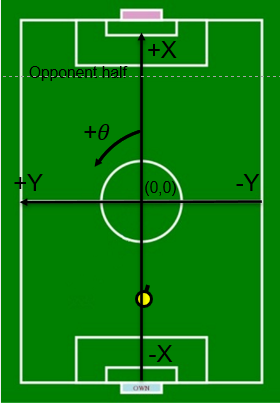
\includegraphics[width=\linewidth]{figures/FCS_field_view.png}
        \small (a) Field Coordinate System (FCS).
    \end{minipage}
    \hspace{0.05\textwidth}
    \begin{minipage}[t]{0.42\textwidth}
        \centering
        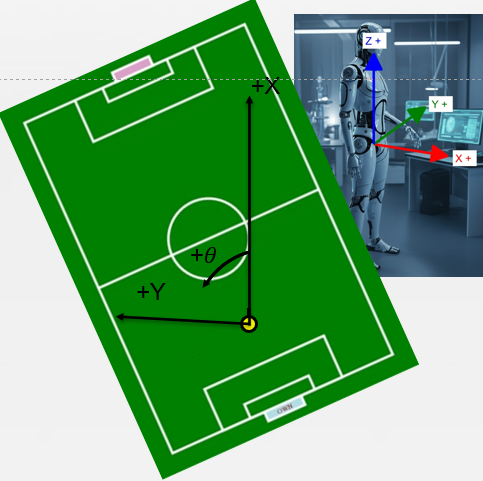
\includegraphics[width=\linewidth]{figures/RCS_field_view.png}
        \small (b) Robot Coordinate System (RCS).
    \end{minipage}
    \caption{Coordinate systems used in the paper. In FCS, the origin is the center of the field, $+X$ points toward the opponent goal, $+Y$ points left, and $\theta=0$ rad points toward the opponent goal. In RCS, the origin is the robot center, $+X$ points forward from the robot perspective, $+Y$ points to the robot's left, and $\theta=0$ rad points straight forward.}
    \label{fig:appendix-coordinate-systems}
\end{figure}

In FCS, robot pose and known landmark positions are expressed in field coordinates. The point $(0,0)$ is the center point of the field. The $+X$ direction points toward the opponent goal, and $+Y$ points to the left. The orientation angle $\theta$ is expressed in radians; $\theta=0$ points toward the opponent goal, and positive rotation is toward the left.

In RCS, observations are expressed from the robot's perspective. The origin is the center of the robot. The $+X$ direction points forward, and $+Y$ points to the robot's left. The angle convention is again in radians, with $\theta=0$ straight ahead and positive rotation toward the left. 

With these conventions, the RCS-to-FCS translation used for motion observations is
\begin{equation}
    \begin{bmatrix}
        v_x^{\mathrm{FCS}} \\
        v_y^{\mathrm{FCS}} \\
        \omega^{\mathrm{FCS}}
    \end{bmatrix}
    =
    \begin{bmatrix}
        \cos\theta_r & -\sin\theta_r & 0 \\
        \sin\theta_r & \cos\theta_r & 0 \\
        0 & 0 & 1
    \end{bmatrix}
    \begin{bmatrix}
        v_x^{\mathrm{RCS}} \\
        v_y^{\mathrm{RCS}} \\
        \omega^{\mathrm{RCS}}
    \end{bmatrix}.
    \label{eq:fcs-rcs-motion-transform}
\end{equation}

The landmark observation model translates a candidate robot pose in FCS and a known landmark position in FCS into the expected landmark observation in RCS. The inputs are
\begin{equation}
    \mathrm{robot}_{\mathrm{FCS}}
    =
    \begin{bmatrix}
        x_r \\
        y_r \\
        \theta_r
    \end{bmatrix},
    \qquad
    \ell_{\mathrm{FCS}}
    =
    \begin{bmatrix}
        x_l \\
        y_l
    \end{bmatrix}.
    \label{eq:landmark-inputs-fcs}
\end{equation}

The corresponding FCS-to-RCS landmark prediction is
\begin{equation}
    \begin{bmatrix}
        x_{pl} \\
        y_{pl} \\
        \theta_{pl}
    \end{bmatrix}
    =
    \begin{bmatrix}
        \cos\theta_r (x_l-x_r) + \sin\theta_r (y_l-y_r) \\
        -\sin\theta_r (x_l-x_r) + \cos\theta_r (y_l-y_r) \\
        \operatorname{atan2}(y_{pl},x_{pl})
    \end{bmatrix}.
    \label{eq:fcs-to-rcs}
\end{equation}

Because the soccer field and coordinate conventions are known, the corresponding landmark Jacobian with respect to the pose components $(x_r,y_r,\theta_r)$ is calculated directly as
\begin{equation}
    J_\ell
    =
    \begin{bmatrix}
        -\cos\theta_r & -\sin\theta_r & y_{pl} \\
        \sin\theta_r & -\cos\theta_r & -x_{pl} \\
        \dfrac{y_l-y_r}{(x_l-x_r)^2+(y_l-y_r)^2}
        &
        -\dfrac{x_l-x_r}{(x_l-x_r)^2+(y_l-y_r)^2}
        &
        -1
    \end{bmatrix}.
    \label{eq:landmark-jacobian}
\end{equation}
This Jacobian is the term $\partial_{\mu_g}\tilde{g}(\tilde{\mu}_g)$ in Eq.~\ref{eq:slide15-generic-update}. It propagates landmark prediction errors back to the field-pose belief.

To clarify, $x_r$, $y_r$, and $\theta_r$ are the current belief
estimates of the robot pose; all transformations and the Jacobian
above are evaluated using these estimates, without access to the
actual robot pose.

\FloatBarrier

\section{Tracking Error for Different Landmark Configurations}
\label{sec:appendix-landmark-tracking}

This appendix provides a more detailed view of the tracking behavior evaluated in Section~\ref{subsec:experiments-visibility-stress}, how landmark availability affects tracking
error over time. 


\begin{figure}[htbp]
    \centering

    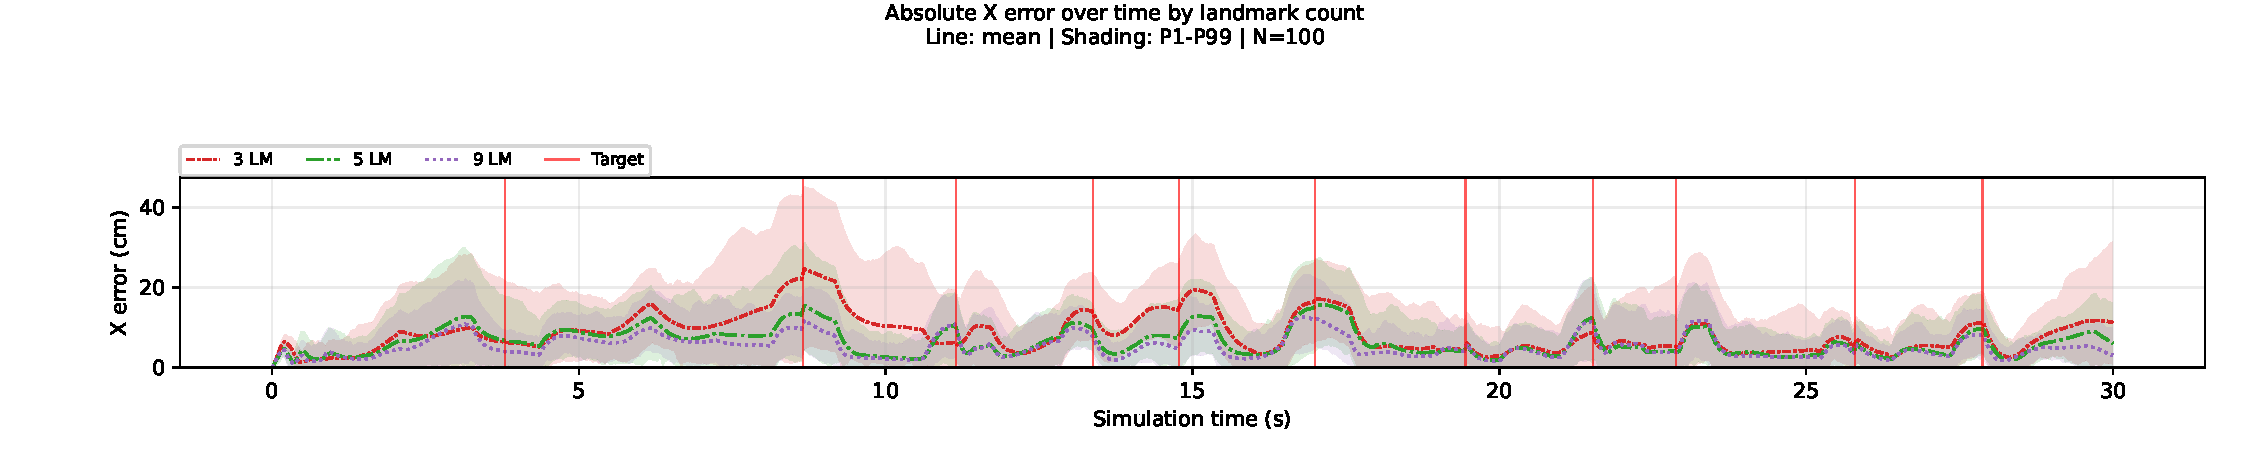
\includegraphics[width=\linewidth,page=1]
    {figures/paper_lm_dataset_20260918_111044_227495_graph.pdf}\\
    {\small (a) Absolute $x$-position error}

    \medskip

    \includegraphics[width=\linewidth,page=2]
    {figures/paper_lm_dataset_20260918_111044_227495_graph.pdf}\\
    {\small (b) Absolute $y$-position error}

    \medskip

    \includegraphics[width=\linewidth,page=3]
    {figures/paper_lm_dataset_20260918_111044_227495_graph.pdf}\\
    {\small (c) Absolute heading error}

    \caption{\scriptsize
    Each landmark configuration (3: two goals and the middle circle; 5: additionally, the two halfway-line boundary points; 9: additionally, the four corners) is evaluated over 100 trials of 30 seconds. All 100 trials for every landmark configuration use identical initial actual and belief poses and replay the same randomly generated target sequence. The trials use the same noise, dropout, field-of-view, and temporary-obstruction settings as Section~\ref{subsec:experiments-visibility-stress}. Landmark counts describe the available map; the number observed at each timestep may be smaller due to the 110 degrees field-of-view. Panels show absolute errors in (a) $x$ position, (b) $y$ position, and (c) heading. Lines show the mean absolute belief-minus-actual error across trials at each timestep; shaded regions span the 1st to 99th percentiles. Heading error is the absolute wrapped angular difference. Thin red vertical lines indicate activation of the next random target.}
    \label{fig:landmark-tracking-error}
\end{figure}
\FloatBarrier

\end{document}
